%&LaTeX
\documentclass[a4paper,12pt,man,english]{apa} % nobf, doc, apa

\usepackage[english]{babel} % ik krijg anders foute citaties...in Zweeds formaat???

\usepackage[]{amsmath, amsfonts, amstext, amsthm}
\usepackage{amssymb}
\usepackage[]{graphics}
\usepackage{graphicx}
\usepackage{epsfig}
\usepackage{epstopdf}

\newcommand{\citep}{\cite}
\newcommand{\citet}{\citeA}
\newcommand{\mat}{\mathbf}
\newcommand{\vc}{\mathbf}

\newcommand{\pkg}{\texttt}
\newcommand{\code}{\texttt}

\renewcommand{\baselinestretch}{2}

\title{A Framework for Discrete Change}

\twoauthors{Ingmar Visser \& Brenda R. J. Jansen}{Maarten Speekenbrink}

\date{\today}

\twoaffiliations{Department of Psychology, University of Amsterdam}{Department of Cognitive, Perceptual and Brain Sciences, University College London}

\note{Correspondence concerning this article should be addressed to:
 \\
 Ingmar Visser \\
 Department of Psychology, University of Amsterdam \\
 Roetersstraat 15 \\
 1018 WB Amsterdam \\
 phone: +31 (20) 5256723 \\
 fax: +31 (20) 6390279 \\
 email: i.visser@uva.nl}


\shorttitle{Modelling Discrete Change}

\abstract{A class of models is developed for measuring and detecting
discrete change in learning and development.  The basic model for
detecting such change is the latent or hidden Markov model.
Traditionally, these models were restricted to categorical, mostly
binary, observed variables, placing severe restrictions on possible
measurement models.  In this paper, the basic model is extended to
include arbitrary distributions for the observed variables, including
multi-variate distributions.  Moreover, there is optional support to
include time-varying predictors.  In effect, this model consists of
mixtures of generalized linear models with Markovian dependencies over time
to model the change process.  In addition, transition parameters can
be made to depend on covariates as well, such that the switching
regime between states depends on characteristics of the individual or
the experimental situation.  The model is illustrated with an example
of participants' learning in the Iowa Gambling Task and in the Weather 
Prediction Task.}


\begin{document}
\maketitle

% intro
Discrete change frequently occurs in learning and development: in
learning concepts, in performance on Piagetian tasks, in
discrimination learning and in conditioning.  This chapter is
concerned with detecting the nature and time points of change in (individual)
time series.  We present a framework of dependent mixture models that can
be used to differentiate between gradual and discrete learning events
in individual time series data.  Before presenting the model in formal
terms and providing some illustrations, we first review some examples
in which discrete change is found.

% phenomena of discrete change in development/learning
Piagetian developmental theory assumes step-wise changes in the
strategies that children apply in all kinds of tasks such as the
conservation learning and the balance scale task (REFERENCE??).
\citet{Maas1992} developed a catastrophe model to describe step-wise
changes or phase transitions in learning and developmental processes.
They applied the catastrophe model to learning in the conservation of
liquid task (REFERENCE??)  in which children have to judge relative
volumes of liquid in glasses of different heights and widths.  Young
children tend to ignore the width dimension and hence always choose
the glass with the highest level of liquid (REFERENCE??).
\citet{Maas1992} showed that there is a sudden transition to a new
strategy in which the children also take the width of the glasses into
account when judging the volume of liquids.

% balance scale rules
\citet{Jansen2001} applied the catastrophe model to
development of strategies on the balance scale task (Siegler, 1981).
In the balance scale task participants have to judge which side of a
balance goes down when the number of weights and their distances to
the fulcrum are varied over trials.  Younger children tend to ignore
the distance dimension in this task, and instead focus solely on the
number of weights on each side of the fulcrum.  This strategy for
solving balance scale items is called Rule 1 \cite{Siegler1981}.  Older
children include the distance dimension in determining their response
to balance scale problems; however, they only do so when the weight
dimension does not differ between the sides of the balance, i.e., when
the number of weights is equal on both sides of the balance scale.
This strategy is called Rule 2 \cite{Siegler1981}.

% hysteresis on the balance scale
\citet{Jansen2001} found clear evidence for stage-wise
transitions between Rule 1 and Rule 2 by testing criteria that were
derived from the catastrophe model.  In particular, she found bimodal
test scores and inaccessibility.  The latter means that there are no
in-between strategies: children apply either Rule 1 or Rule 2 and
there is no in-between option.  \citet{Jansen2001} also found
evidence for hysteresis: the phenomenon that switching between
strategies is asymmetric.  Children can switch from Rule 1 to Rule 2
and back, but this occurs at different trials.  In particular, if the
distance dimension in the balance scale problems is made more salient
by increasing the distance difference between weights on either side
of the balance scale, children may switch from Rule 1 to Rule 2.  If
subsequently the distance difference is decreased again, children may
switch back to using Rule 1.  Hysteresis is the phenomenon that this
switch back occurs at a different value of the control variable, in
this case the distance difference.

% conditioning and addiction research
Also in animal learning and conditioning, evidence is found for sudden
changes in response behavior \cite{Gallistel2004}.  In particular, in
their study, evidence was found for sudden onset of learning: at the
start of the learning experiment, pigeons did not learn anything
and performance was stable; after a number of trials, learning kicked
in and there were large increases in performance.  \citeauthor{Gallistel2004} 
focused on modeling the distribution of onset times: that is, the trials at
which learning suddenly takes off.  A similar interest in process
onset times is found in addiction research.  For example,
\citet{Sher2004} study the age at which children start using alcohol
and how this related to eventual outcomes in terms of addiction.

% discrimination and categorization learning
Sudden transitions in learning are also observed in simple
discrimination learning paradigms in which participants learn to
discriminate a number of stimuli based on a single dimension such as
form or color.  This kind of learning is referred to as all-or-none
learning or concept identification learning.  \citet{Raijmakers2001}
found evidence for different strategies applied by children when faced
with such a learning task.  \citet{Schmittmann2006} reanalyzed their
data using hidden Markov models to show that both strategies are
characterized by sudden transitions in the learning process.

% latent Markov versus time series analyses/outline
In above mentioned applications, the data consist mostly of a few
repeated measurements administered to large groups of participants.
The focus in the current chapter is rather on data that consist of
many repeated measurements, or time series, observed in only a few
participants or even just a single participant.  For example,
\citet{Visser2009} analyzed data from a single participant in an
experimental task that manipulates the trade-off between speed and
accuracy.  The data consisted of three time series with each around
150 repeated measurements of both reaction time and accuracy.  Below
we provide examples of analyzing time series from single participants
from two experiments; one from the Iowa Gambling Task and one from the
Weather Prediction Task.  The interest in these tasks is to show that
participants develop different strategies over time in responding to
the stimuli and that the transition from one strategy to the next is a
discrete event.  Before providing these illustrations, below we give a
formalization of dependent mixture models and a brief overview of the
\pkg{depmixS4} package that was developed to specify and fit such models.


\section{Dependent Mixture Models}

% outline
In this section we describe a class of models which are especially
suitable for describing and testing discrete change in (individual)
time series data.  The dependent mixture model is similar to, but
slightly different from, two other types of models that are in use for
modelling discrete change: the hidden and the latent Markov models.

% history of Markov models/LMM applications
Markov models have been used extensively in the social sciences; for
example, in analyzing language learning \cite{Miller1952,Miller1963} and
in the analysis of paired associate learning \cite{Wickens1982}.  In
these models, the focus is on survey type data: a few repeated
measurements taken in a large sample.  \citeA{Langeheine1990} discuss
latent Markov models and their use in sociology and political science
(see also McCutcheon, 1987).  Latent transition models have been used
in studying development of math skills \citep{Collins1992} and in
medical applications \citep{Reboussin1998}; \citet{Kaplan2008}
provides an overview of such models, that are called stage-sequential
models in the developmental psychology literature.

\nocite{McCutcheon1987}

% hidden Markov models
Hidden Markov models (HMM) tend to be used in the analysis of long
univariate (individual) timeseries.  For example, HMMs are the model
of choice in speech recognition applications \cite{Rabiner1989}.  In
biology, HMMs are used to analyze DNA sequences \cite{Krogh1998} and
in econometric science, to analyze changes in stock market prices and
commodities \cite{Kim1994}.

% depmix model
The dependent mixture model that we propose here spans the range from
latent Markov models for few repeated measurements with many
participants to hidden Markov models for individual time series.  In
addition, the dependent mixture model includes multivariate responses.
The dependent mixture model consists of the following elements:
\begin{enumerate}
	\item $S$ is a collection of discrete states
	\item $S_{t} = \mat{A}S_{t-1}+\xi_{t}, \mat{A}$, a transition matrix
	\item $O_{t} = \mat{B}(S_{t}) + \zeta_{t}, \mat{B}$,  an observation density
\end{enumerate}
Here $\xi_{t}$ and $\zeta_{t}$ are independent error processes 
\cite{Elliott1995}. 

% state space
The state space, which is a set of discrete states, captures the
different states that the learning or developmental process under
consideration can be in.  In the balance scale example mentioned
above, children are applying one of two possible strategies in
responding to the items.  The states are characterized by their
corresponding observation densities.  Using for example Rule 1 in the
balance scale task leads to correct answers on some items and
incorrect answers on others.  A different strategy may lead to correct
answers on some items and to guessing behavior on other items.  In
analyzing categorization learning data, in which participants learn to
categorize a set of objects, a typical initial state is that
participants are guessing because at the start of the task they have
no knowledge of which features are important in categorization.
Hence, the states in the state space represent knowledge states of the
participants, such that different knowledge states lead to different
observed behavior or responses.

% transitions/matrix
The transition matrix $\mat{A}$ describes the transitions between
states over repeated measures or trials.  This matrix summarizes the
probabilities of transitioning from one state to another which
represents learning or development.  The transition model contains the
Markov assumption:
$$Pr(S_{t}|S_{t-1}, \ldots, S_{1}) = Pr(S_{t}|S_{t-1}),$$
which means that the current state (at time $t$) only depends on the
previous state $S_{t-1}$, and not on earlier states.

% observation densities
The observation densities $\mat{B}$ form the measurement part of the
model; these describe the distributions of the observations
conditional on the current state. Hence, these distributions
characterize the state, and in our examples, these characterize the
strategy that a participant is using at a given measurement occasion.

% log-likelihood
The log-likelihood of DMMs is usually computed by the
so-called forward-backward algorithm \citep{Baum1966,Rabiner1989}, or
rather by the forward part of this algorithm.  \citet{Lystig2002}
changed the forward algorithm in such a way as to allow computing the
gradients of the log-likelihood at the same time.  They start by
rewriting the likelihood as follows (for ease of exposition the
dependence on the model parameters is dropped here):
\begin{equation}
	L_{T} = Pr(\vc{O}_{1}, \ldots, \vc{O}_{T}) = \prod_{t=1}^{T}
Pr(\vc{O}_{t}|\vc{O}_{1},
	\ldots, \vc{O}_{t-1}),
	\label{condLike}
\end{equation}
where $Pr(\vc{O}_{1}|\vc{O}_{0}):=Pr(\vc{O}_{1})$. Note that for a
simple, i.e.\ observed, Markov chain these probabilities reduce to
$Pr(\vc{O}_{t}|\vc{O}_{1},\ldots,
\vc{O}_{t-1})=Pr(\vc{O}_{t}|\vc{O}_{t-1})$.
The log-likelihood can now be expressed as:
\begin{equation}
	l_{T} = \sum_{t=1}^{T} \log[Pr(\vc{O}_{t}|\vc{O}_{1}, \ldots,
\vc{O}_{t-1})].
	\label{eq:condLogl}
\end{equation}

To compute the log-likelihood, \citet{Lystig2002} define the following
(forward) recursion:
\begin{align}
	\phi_{1}(j) &:= Pr(\vc{O}_{1}, S_{1}=j) = \pi_{j} b_{j}(\vc{O}_{1})
	\label{eq:fwd1} \\
\begin{split}
	\phi_{t}(j) &:= Pr(\vc{O}_{t}, S_{t}=j|\vc{O}_{1}, \ldots,
\vc{O}_{t-1}) \\
	&= \sum_{i=1}^{N} [\phi_{t-1}(i)a_{ij}b_{j}(\vc{O}_{t})] \times
(\Phi_{t-1})^{-1},
	\label{eq:fwdt}
\end{split}
\end{align}
where $\Phi_{t}=\sum_{i=1}^{N} \phi_{t}(i)$. Combining
$\Phi_{t}=Pr(\vc{O}_{t}|\vc{O}_{1}, \ldots, \vc{O}_{t-1})$, and
equation~(\ref{eq:condLogl}) gives the following expression for the
log-likelihood:
\begin{equation}
	l_{T} = \sum_{t=1}^{T} \log \Phi_{t}.
	\label{eq:logl}
\end{equation}

Note that so far no assumptions have been made about the response
distributions $b_{j}$, hence these can be arbitrary univariate or
multivariate distributions.


\section{DepmixS4}

% outline/abstract: this has redundant information, mostly discussed
% in detail below
\pkg{depmixS4} implements a general framework for defining and fitting
dependent mixture models in the R programming language \citep{R2008}.
This includes standard Markov models, latent/hidden Markov models, and
latent class and finite mixture distribution models.  The models can
be fitted on mixed multivariate data with multinomial and/or gaussian
distributions.  

% design goals
The \pkg{depmixS4} package was motivated by the fact that Markovian
models are used commonly in the social sciences, but no comprehensive
package was available for fitting such models in R. Common programs
for Markovian models include Panmark \citep{Pol1996}, and for latent
class models Latent Gold \citep{Vermunt2003}.  Those programs are
lacking a number of features that were needed in our research.  In
particular, \pkg{depmixS4} was designed to meet the following goals:
\begin{enumerate}

	\item to be able to fit transition models with covariates, i.e.,
	to have time-dependent transition matrices.

	\item to be able to include covariates in the prior or initial
	state probabilities of models.

	\item to allow for easy extensibility; in particular, to be able
	to add new response distributions, both univariate and
	multivariate, and similarly to be able to allow for the addition
	of other transition models, e.g., models for observations in 
	continuous time. 

\end{enumerate}

Although \pkg{depmixS4} is designed to deal with longitudinal or time
series data, for say $T>100$, it can also handle the limit case with
$T=1$ in analyzing cross-sectional data.  In those cases, there are no
time dependencies between observed data, and the model reduces to a
finite mixture model \cite{McLachlan2000}, or a latent class model
\cite{McCutcheon1987}.  Although there are other specialized (R)
packages to deal with mixture data, these don't allow the inclusion of 
covariates on the prior probabilities of class membership.

\pkg{depmixS4} is built using S4 classes (object oriented classes in R)
to allow easy extensibility (Chambers, 1998). A depmix model consists 
of the following: 
\begin{enumerate} 
	\item A model for the initial or prior probabilities 
	\item A list of transition models; one model for each row of the 
	transition matrix
	\item A list of response models for each of the states of the model; 
	this is a list of lists in the case of multivariate responses. 
\end{enumerate} 
Each of these are adressed briefly below. 


\subsection{Transition and prior probabilities models}

% transition and initial state probs
By default, each row of the transition matrix and the vector of initial state 
probabilities is modelled as a baseline-category multinomial logistic 
model \cite<see>[chapter 7]{Agresti2002}. This means that covariates 
can be used as predictors in these models. In particular, the model 
for each multinomial is:
\begin{equation} 
	\pi_{i} = \frac{\exp(\alpha_{i}+\mathbf{\beta}^{`}_{i}\vc{x})}
				{1+\sum_{j=1}^{J-1}\exp(\alpha_{j}+\mathbf{\beta}^{`}_{j}\vc{x})},
\end{equation}
where $\pi_{i}$ is the probability (e.g.\ the probability of the
$i$-th initial state); the $\alpha_{i}$ are the category intercepts;
the $\mathbf{\beta}_{i}$ are the category regression coefficients;
$\vc{x}$ is a vector of covariates or predictors; $J$ is the number
of states; in this example, $J$ serves as the baseline-category,
meaning that $\alpha_{J}$ and $\mathbf{\beta}_{J}$ are zero. 


\subsection{Response models}

% response models
Response models in \pkg{depmixS4} interface with the \code{glm} 
functions available in R and with the \pkg{nnet}-package for the 
multinomial logistic models. Normally distributed data can hence be 
modelled with direct effects included as well. For example, normal 
data are modelled as:
\begin{equation}
	O_{t}|S_{t} = \mu + \mathbf{\beta}^{`}\vc{x} + \epsilon_{t},
\end{equation}
where $\mu$ the (state-dependent) mean; $\vc{x}$ is a vector of
covariates or predictors; $\mathbf{\beta}$ is the vector of
(state-dependent) regression coefficients; $\epsilon_{t}$ is a
normally distributed error with (state-dependent) standard deviation
$\sigma$.

Multinomial responses are modeled by the same multinomial 
baseline-category logistic model as is used for the transition 
probabilities and the initial state probabilities. Other response 
functions from the generalized linear model family that can be used 
include: binomial logistic regression, poisson regression, gamma and 
inverse gaussian. There is also support for the multivariate normal 
distribution. 

% MAARTEN: de multinomial logistic models maken weer gebruik van andere
% packages toch, kun je daar de referentie van geven?


\subsection{Parameter Estimation}

Parameters are estimated in \pkg{depmixS4} using the EM algorithm or
through the use of a general Newton-Raphson optimizer.  EM is used by
default in unconstrained models, but otherwise direct optimization is
done using \pkg{Rdonlp2} \cite{Tamura2007,Spellucci2002}, because it
handles general linear (in)equality constraints, and optionally also
non-linear constraints.


\section{Illustrations}

% \subsection{Toy data: parameter retrieval} ????

Two illustrations are provided below of models that analyze single
participant time series data from two common experimental paradigms.
In both of these, participants learn different strategies through
trial and error.


\subsection{Iowa gambling task}

% what is the IGT?
The Iowa gambling task (IGT) is an experimental paradigm designed to
mimic real-life decision-making situations \cite{Bechara1994}, in the
way that it factors uncertainty, reward and punishment
\cite{Dunn2006}.  The task requires the selection of cards from four
decks.  Each deck is characterized by a certain amount of gain
(delivered on each draw), frequency of loss, and amount of loss.  Two
decks (A and B) yield consistently high rewards, but also high,
probabilistic penalties and are both (equally) disadvantageous in the
long run.  The other two decks (C and D) yield consistently smaller
rewards, but also low, probabilistic penalties and are both (equally)
advantageous in the long run.  It is assumed that the ventromedial
prefrontal cortex (VMPFC) is active in the IGT as VMPC patients show
impaired task performance.  Their preference for the decks with
immediate high rewards indicates ``myopia for the future''.

% what is the HDT? developmental trends and relevance?
\citet{Crone2004} designed a developmentally appropriate analogue of
the IGT, the Hungry Donkey Task (HDT), with a similar win and loss
schedule although the absolute amounts were reduced by a factor of 25.
The HDT is a pro-social game inviting the player to assist a hungry
donkey to collect as many apples as possible, by opening one of four
doors.  Again, doors A and B are characterized by a high constant gain
(10 apples), whereas doors C and D deliver a low constant gain (2
apples).  At doors A and C, a loss of 50 apples (A) or 10 apples (C)
is delivered in 50\% of the trials.  For doors B and D, frequency of
loss is only 10\%.  The median loss of doors B and D is 10 and 2,
respectively.  \citet{Crone2004} administered the HDT to children from
four age groups (6-9, 10-12, 13-15, and 18-25 year-olds) and concluded
that children also fail to consider future consequences.

% strategic reanalysis of the HDT: different strategies found by
% finite mixture analysis
A reanalysis of this dataset \cite{Huizenga2007} indicated that
participants might solve the task by sequentially considering the
three dimensions (constant gain, frequency of loss, and amount of
loss) in order to choose a door.  The youngest children in the
dataset mostly seem to focus on the dominant dimension in the task, frequency
of loss, resulting in equal preference for doors B and D. Older
participants seem to use a two-dimensional rule where participants
first focus on the frequency of loss and then consider amount of loss,
resulting in a preference for door D. A third very small subgroup
seems to use an integrative rule where participants combine all three
dimensions in the appropriate way.  Participants using the integrative
rule pick cards from doors C and D, which are advantageous in the long
run.

% problematic aspects of standard analysis
Typical analyses of these data use the last 60 trials in a series of
200 trials.  A silent assumption made in these analyses is
that behavior has stabilized after 140 learning trials; this could
very well be wrong and it is highly likely that there are individual
differences in this learning process.

% proposed analysis here
Here, we analyze IGT learning data from a single participant with the aim to
establish 1) at which trial learning stops, i.e., at which
trial behavior has stabilized, and 2) what strategies participants use
during and at the end of learning.  Models with an increasing number
(from 2 through 5) of latent states were fitted to the time series of
various participants.  The responses were fitted with multinomial
logistic models for the 4 possible choices that participants make in
this task.  There were no covariates on any of the parameters.  The
only constraint imposed on the models' parameters was that
there were designated begin and end states.  This means that the
initial state probabilities were fixed to one for the first state and
to zero for the remaining states.  For the transition matrix this means
that the final state was an absorbing state: the probability of
transitioning out of that state is zero.  This was done to ensure that
there would be a final state in which participants end which provides
the possibility of immediately seeing participants' behavior at the
end of the task.  Models were selected using the Akaike Information
Criterion (AIC; Akaike, 1973).

\nocite{Akaike1973} % check the year!!

%We chose to analyze two participants that used different strategies at
%the end of the task as analyzed in the manner proposed by
%\citet{Huizenga2007}.  The first participants' data 
The data were best 
described by a 4-state model.  This model's transition matrix is:
$$
\mat{A} = \begin{pmatrix} 
				0.64 & 0.33 & 0.00 & 0.03 \\
				0.10 & 0.89 & 0.01 & 0.00 \\
				0.05 & 0.00 & 0.95 & 0.00 \\
				0.00 & 0.00 & 0.00 & 1.00
		  \end{pmatrix}
$$
As can be seen from the transition matrix the final state is
absorbing.  States 2 and 3 are also fairly stable with high diagonal
probabilities of 0.89 and 0.95 respectively.  The response parameters
are presented in Table~\ref{tab:igt4} below.

\begin{table}
	\caption{Estimates for the Iowa Gambling Task model}
	\label{tab:igt4}
	\begin{tabular}{lcccccccc} \hline
		state & p(A) & p(B) & p(C) & p(D) \\
		$S_1$ & 0    & 0.06 & 0.31 & 0.63 \\
		$S_2$ & 0.33 & 0.67 & 0    & 0 \\ 
		$S_3$ & 0    & 0    & 1    & 0 \\
		$S_4$ & 0    & 0.06 & 0.94 & 0 
	\end{tabular}
\end{table}

The states have clear interpretations. States 3 and 4 are both
dominated by C responses, and state 4 has a low probability of B
responses. States 1 and 2 are dominated C and D and A and B responses 
respectively. To get a clearer interpretation of these states it is
necessary to consider when they are visited during the learning
process. The Viterbi algorithm (REFERENCE) provides us with the
posterior state sequence, i.e., the sequence of states that the
participant is in at each trial. This sequence is depicted in
Figure~\ref{fig:post4}. 

\begin{figure}
\begin{center}
	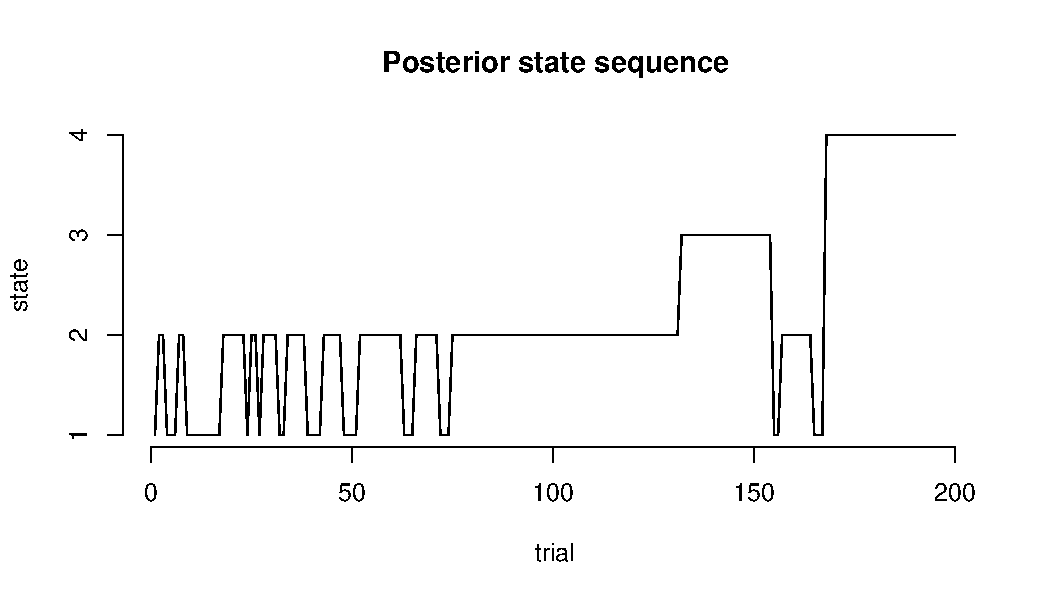
\includegraphics[width=\textwidth]{graphs/post4.pdf}
	\label{fig:post4}
	\caption{Posterior state sequence for the 4 state model.}
\end{center}
\end{figure}

At the start of training there are many switches between states 1 and 
2, indicating that behavior is mostly random choices between all four 
categories, albeit with a slight preference for B and D over A and C
choices. This preference indicates a focus on the frequency of loss
associated with each of the doors as B and D have low frequency of
loss. After this, there is a period of stable state 2 behavior
associated with responses A and B. After that there is stable state 3 
behavior, consisting only of C responses, a short transitional period 
and then state 4 behavior consisting of 94 \% C choices and some B
choices, i.e., almost optimal behavior. The choice proportions and the
model predicted choice proportions are depicted in
Figure~\ref{fig:igt4}. 

\begin{figure}
\begin{center}
	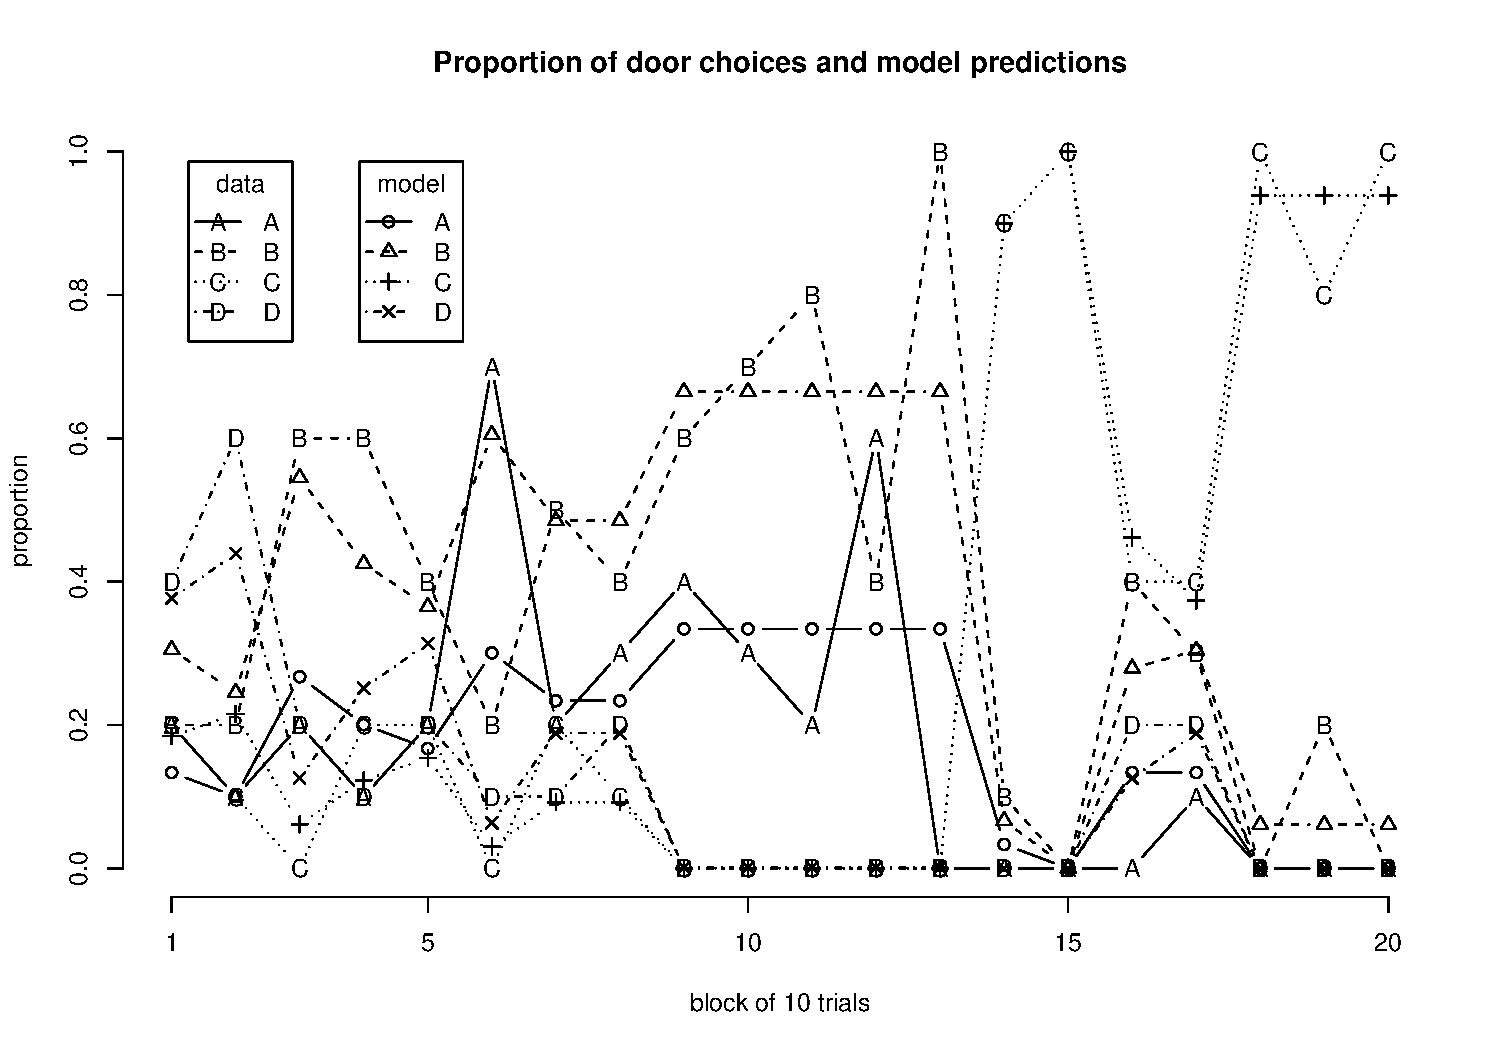
\includegraphics[width=\textwidth]{graphs/igt4.pdf}
	\label{fig:igt4}
	\caption{Data and model predicted proportions of door choices in
	the IGT.}
\end{center}
\end{figure}

The initial preference for B and D choices confirms the theory
expressed in \citet{Huizenga2007} that frequency of loss is the
dominant dimension in the IGT. The final states with mostly C 
choices represents one of the optimal strategies, which consists of
both C and D responses. Note that both C and D responses generate equal
profits in the long run. 


\subsection{Weather prediction task}

%Still to add models and data.

The Weather Prediction Task \cite<WPT>{Knowlton1994} %(WPT, Knowlton, Squire \& Gluck, 1994) 
is
a probabilistic categorization task in which participants learn to
predict (or categorize) the state of the weather (sun or rain) on the
basis of four ``tarot'' cards (cards with abstract geometrical
patterns).  On a given trial, one, two, or three cues are present.
There are a total of 14 possible cue patterns, and each one is
associated with a particular probability distribution over the states
of the weather.  In order to perform in the task, participants must
predict the weather in accordance with these conditional
probabilities.

\nocite{Knowlton1994}

%The WPT has been popular in neuropsychological research,
%particularly because amnesic patients perform this task rather
%well, despite not being able to remember actually many aspects
%of the task (or in some cases, even performing the task at all).
%This has led to the conclusion that probabilistic category learning
%depends on implicit memory, which is separate from explicit
%memory. While this conclusion is debatable (Speekenbrink, Channon
%\& Shanks, 2008), the finding of relatively unimpaired performance
%by amnesic individuals remains striking.

There are different accounts of probabilistic category learning 
\cite<see e.g.>[for an overview]{Ashby2005}.
According to instance or exemplar learning theories, participants
learn by storing each encountered cue-outcome pair.  When presented
with a probe cue pattern, a response is made by retrieving these 
exemplars are retrieved from memory and weighting them according 
to their similarity to the probe cue pattern. According to associative theories,
participants learn by gradually associating the individual
cues (or cue patterns in configural learning) to the outcomes. Finally, in
rule-learning, participants are taken to extract rules by which to
categorize the different cue patterns.  \cite{Gluck2002} proposed a
number of such rules (or strategies). The rules differ in the way
the cues are combined into a response. A main difference is whether responses are
based on the presence/absence of a single cue, or whether information 
from multiple cues is integrated. \citeauthor{Gluck2002}
formulated all strategies in a deterministic and optimal manner (e.g., 
the multi-cue strategy corresponded to giving the optimal response to
each cue pattern). \citet{Meeter2006}  allowed for probabilistic
responding (a small probability of responding non-optimally) as well
as switches between strategies during learning. However, both strategies 
and response probabilities remained predefined. Alternative non-strategy based 
analyses of the WPT \cite{Lagnado2006,Speekenbrink2008} have estimated 
response strategies through logistic regression, allowing the regression 
coefficients to change smoothly over time.

%associative, rule-based.
Here, we combine the regression and strategy-based approaches, and analyse 
the behavior of a single individual performing the
WPT for 200 trials.  We are particularly interested
in evidence for strategy switching and whether a DMM can recover
strategies in accordance with \citeA{Gluck2002}. We chose to analyse the 
``average'' participant (the participant with performance closest to 
the group average) in a large unpublished dataset. We let each state 
be characterized by a GLM with a Binomial distributed response and 
logistic link function (i.e., a logistic regression model). The regression
coefficients of a model relating the cues to the state of the weather are 
given in column ```validity'' of Table~\ref{tab:WPT}. Note that indentical
coefficients for the model relating the cues to responses would indicate 
probability matching. A maximizing strategy is indicated by more
extreme regression coefficients.

As we fitted a DMM to the data of a single subject, it was necessary
to place some constraints on the model.  Specifically, we constrained
the state transitions to be in a ``left-right'' format (states can
only proceed to the immediately adjacent state and never back, and
must start in the initial state).  We fitted a single, two and three
state model to the data.  This showed that a two state model was
better than a single or three state model.

\begin{table}
\caption{Estimates for the weather prediction task}
\label{tab:WPT}
\begin{tabular}{lcccccccccc} \hline
 & & \multicolumn{1}{c}{} && \multicolumn{1}{c}{1 state} & & \multicolumn{2}{c}{2 state} &&
 \multicolumn{2}{c}{2 state (constr.)} \\ \cline{5-5} \cline{7-8} \cline{10-11}
parameter && validity && $S_1$ & & $S_1$ & $S_2$ & & $S_1$ & $S_2$ \\ \hline
(intercept) && 0 && -0.69 & & -2.73 & 0.88 & & -1.24 & 0 \\
cue 1 && 2.10 && 1.69 && 2.12 & 1.60 && 1.65 & 1.97 \\
cue 2 && 0.58 && 1.12 && 0.97 & 1.63 && 0 & 1.92 \\
cue 3 && -0.58 && -0.49 && 0.91 & -2.03 && 0 & -1.58 \\
cue 4 && -2.10 && -1.32 && 0.69 & -3.16 && 0 & -2.67 \\ \hline
 & & & & \multicolumn{1}{c}{AIC=204.47} & & \multicolumn{2}{c}{AIC=187.50} &&
 \multicolumn{2}{c}{AIC=185.24}
\end{tabular}
\end{table}

Investigation of the parameter estimates (see Table~\ref{tab:WPT})
showed that the regresion coefficient for the first cue was of much
larger magnitude than that of the other cues. As such, the first
state seems representative of single cue strategy.  Alternatively, as
all regression coefficients are positive, it could indicate a
``counting'' heuristic, where the propensity of ``sun'' responses
increases when more cues are present (regardless of which cues they
are).  However, in that case, we would expect the regression
coefficients to be of roughly identical magnitude. The second state
seemed to represent a multi-cue strategy, as all cues had regression
coefficients of reasonable magnitude in the direction of the objective
cue validities.

To reduce the degrees of freedom and improve parameter estimates, we
implemented constraints to force state 1 into a single cue strategy
(fixing the coefficients of the remaining three cues to 0) and state 2
in a multi-cue strategy (forcing the intercept to 0).  These
restrictions resulted in a better AIC value of AIC=185.24 (df=7).
Interestingly, the single cue strategy was somewhat different than
described by \citet{Gluck2002}.  Parameter estimates indicated relatively
more consistent predictions of ``rain'' in the absence of cue 1
($Pr(\text{sun}) = 0.22$) and more inconsistent predictions of ``sun''
in the presence of cue 1 ($Pr(\text{sun}) = 0.60$).  The cue weights
of the multi-cue strategy were in the direction of the optimal
weights.  The Viterbi state sequence indicated that the participant
used the single cue strategy for the first 60 trials, and then
switched to the multi-cue strategy.


\section{Discussion}

General issues
\begin{itemize}
	\item It is feasible to fit hidden Markov models in moderate length individual time series
	\item illustrations show results that are consistent with usual group based analyses AND 
	provide extra information on switching between strategies over the course of learning
	\item Many applications in experimental psychology: examples????
\end{itemize}

Specific insights from the illustrations: suggestions welcome

Analyzing the WPT data on an individual level allowed us to precisely estimate idiographic strategies and their progression during learning. Moreover, using DMMs, we can combine an individual and group level analysis, increasing reliability of the individual analyses whilst allowing for substantial individual differences. Previous analyses \cite<e.g.,>{Meeter2006} pre-defined individual strategies, based on participants' self-reports in \citet{Gluck2002}. Interestingly, \citet{Gluck2002} noted that these self-reports often did not correspond to the strategies evident in participants' responses. It is well known that people may find it difficult to verbalize the way in which they integrate multiple sources of information. As such, estimating strategies directly from participants' responses will result in more valid assessment of their response strategies, and provides a direct test of the validity of the strategy set identified by \citeauthor{Gluck2002}.

Possible future extensions in depmixS4
\begin{enumerate}
	\item richer measurement models, eg factor models, AR models etc
	\item richer transition models, eg continuous time measurement occasions
	\item explicit state durations
	\item identifiability of models
	\item model selection
\end{enumerate}





\section*{Author note}

Ingmar Visser was supported by an EC Framework 6 grant, project 516542
(NEST).  Maarten Speekenbrink was supported by the ESRC Centre for
Economic Learning and Social Evolution (ELSE).  Thanks to Hilde
Huizenga, Brenda Jansen and Anna van Duijvenvoorde for the Iowa
Gambling task data and David Lagnado for the Weather Prediction Task
data.

\bibliography{all,ingmar,individual}

\end{document}















